\documentclass[tikz,border=3pt]{standalone}
\usepackage{xcolor}
\usetikzlibrary{arrows.meta,calc,fit,positioning}

\definecolor{ink}{HTML}{1F2937}
\definecolor{muted}{HTML}{64748B}
\definecolor{line}{HTML}{475569}
\definecolor{panel}{HTML}{F8FAFC}
\definecolor{blue}{HTML}{2F6FA7}
\definecolor{blueSoft}{HTML}{E8F1FB}
\definecolor{green}{HTML}{2E8B57}
\definecolor{greenSoft}{HTML}{E7F4EC}
\definecolor{amber}{HTML}{D98C1F}
\definecolor{amberSoft}{HTML}{FFF1D8}
\definecolor{red}{HTML}{C44E52}
\definecolor{redSoft}{HTML}{FBE7E6}
\definecolor{violetSoft}{HTML}{EFE8FA}

\begin{document}
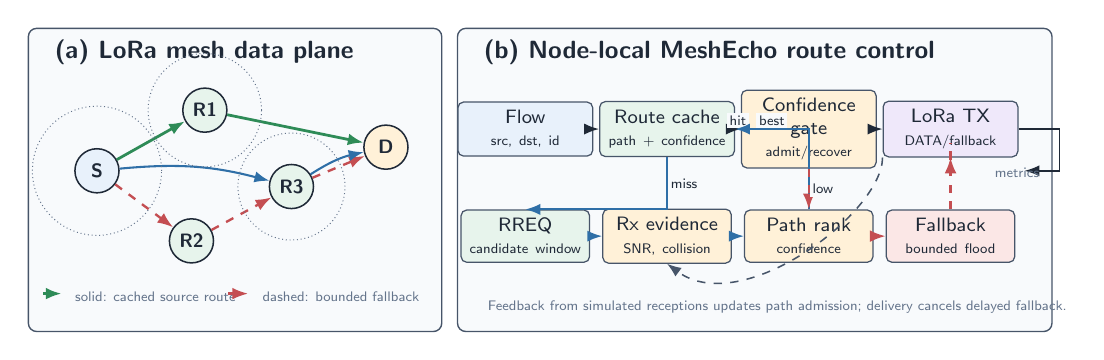
\begin{tikzpicture}[
    font=\sffamily\scriptsize,
    panelbox/.style={
        draw=line,
        fill=panel,
        line width=0.5pt,
        rounded corners=3pt
    },
    nodechip/.style={
        circle,
        draw=ink,
        line width=0.55pt,
        minimum size=0.56cm,
        inner sep=0pt,
        font=\sffamily\scriptsize\bfseries,
        text=ink,
        fill=white
    },
    module/.style={
        draw=line,
        line width=0.45pt,
        rounded corners=2pt,
        minimum height=0.62cm,
        text width=1.42cm,
        align=center,
        inner xsep=3pt,
        inner ysep=3pt,
        text=ink
    },
    wideModule/.style={
        module,
        text width=1.50cm
    },
    route/.style={-{Latex[length=2.0mm]}, draw=green, line width=1.0pt},
    fallback/.style={-{Latex[length=2.0mm]}, draw=red, line width=0.85pt, dashed},
    control/.style={-{Latex[length=1.9mm]}, draw=blue, line width=0.75pt},
    arrow/.style={-{Latex[length=1.9mm]}, draw=ink, line width=0.65pt},
    feedback/.style={-{Latex[length=1.8mm]}, draw=line, line width=0.55pt, dashed},
    label/.style={font=\sffamily\tiny, text=ink, fill=panel, inner sep=1pt}
]

% Panel backgrounds.
\node[panelbox, minimum width=5.25cm, minimum height=3.85cm, anchor=south west] (leftPanel) at (0,0) {};
\node[panelbox, minimum width=7.55cm, minimum height=3.85cm, anchor=south west] (rightPanel) at (5.45,0) {};

\node[anchor=west, font=\sffamily\bfseries\small, text=ink] at (0.22,3.56) {(a) LoRa mesh data plane};
\node[anchor=west, font=\sffamily\bfseries\small, text=ink] at (5.67,3.56) {(b) Node-local MeshEcho route control};

% Left panel: LoRa mesh topology and forwarding modes.
\node[nodechip, fill=blueSoft] (S) at (0.88,2.05) {S};
\node[nodechip, fill=greenSoft] (R1) at (2.25,2.82) {R1};
\node[nodechip, fill=greenSoft] (R2) at (2.08,1.16) {R2};
\node[nodechip, fill=greenSoft] (R3) at (3.35,1.85) {R3};
\node[nodechip, fill=amberSoft] (D) at (4.55,2.35) {D};

\draw[route] (S) -- (R1);
\draw[route] (R1) -- (D);
\draw[fallback] (S) -- (R2);
\draw[fallback] (R2) -- (R3);
\draw[fallback] (R3) -- (D);
\draw[control] (S) to[bend left=10] (R3);
\draw[control] (R3) to[bend left=10] (D);

\draw[draw=muted, line width=0.35pt, densely dotted] (S) circle [radius=0.82cm];
\draw[draw=muted, line width=0.35pt, densely dotted] (R1) circle [radius=0.72cm];
\draw[draw=muted, line width=0.35pt, densely dotted] (R3) circle [radius=0.68cm];

\node[anchor=west, font=\sffamily\tiny, text=muted] at (0.48,0.45) {solid: cached source route};
\draw[route] (0.20,0.49) -- (0.43,0.49);
\node[anchor=west, font=\sffamily\tiny, text=muted] at (2.86,0.45) {dashed: bounded fallback};
\draw[fallback] (2.55,0.49) -- (2.80,0.49);

% Right panel: MeshEcho routing logic.
\node[wideModule, fill=blueSoft] (flow) at (6.32,2.58) {Flow\\{\tiny src, dst, id}};
\node[wideModule, fill=greenSoft] (cache) at (8.12,2.58) {Route cache\\{\tiny path + confidence}};
\node[wideModule, fill=amberSoft] (gate) at (9.92,2.58) {Confidence gate\\{\tiny admit/recover}};
\node[wideModule, fill=violetSoft] (tx) at (11.72,2.58) {LoRa TX\\{\tiny DATA/fallback}};

\node[module, fill=greenSoft] (rreq) at (6.32,1.22) {RREQ\\{\tiny candidate window}};
\node[module, fill=amberSoft] (rx) at (8.12,1.22) {Rx evidence\\{\tiny SNR, collision}};
\node[module, fill=amberSoft] (rank) at (9.92,1.22) {Path rank\\{\tiny confidence}};
\node[module, fill=redSoft] (repair) at (11.72,1.22) {Fallback\\{\tiny bounded flood}};

\draw[arrow] (flow) -- (cache);
\draw[arrow] (cache) -- node[label, above] {hit} (gate);
\draw[arrow] (gate) -- (tx);
\draw[arrow] (tx.east) -- ++(0.52,0) |- (12.66,2.05);
\node[anchor=west, font=\sffamily\tiny, text=muted] at (12.16,2.03) {metrics};

\draw[control] (cache.south) |- node[label, near start, right] {miss} (rreq.north);
\draw[control] (rreq) -- (rx);
\draw[control] (rx) -- (rank);
\draw[control] (rank.north) |- node[label, near end, above] {best} (cache.east);

\draw[fallback] (gate.south) -- node[label, right] {low} (rank.north);
\draw[fallback] (rank) -- (repair);
\draw[fallback] (repair.north) |- (tx.south);
\draw[feedback] (tx.south west) .. controls +(0,-0.70) and +(0.95,-0.70) .. (rx.south);

\node[anchor=west, font=\sffamily\tiny, text=muted] at (5.72,0.32)
    {Feedback from simulated receptions updates path admission; delivery cancels delayed fallback.};

\end{tikzpicture}
\end{document}
